\documentclass[11pt]{article}

\usepackage{fancyhdr}
\usepackage{float}
\usepackage[T1]{fontenc}
\usepackage{graphicx}
\usepackage[utf8]{inputenc}
\usepackage[normalem]{ulem}
\usepackage[svgnames]{xcolor}
\usepackage[paperheight=27.94cm,paperwidth=21.59cm,left=1.9cm,right=1.9cm,top=1.9cm,bottom=1.9cm]{geometry}
\usepackage[hidelinks]{hyperref}
\usepackage{xurl}


\setlength\parindent{0pt}
\renewcommand{\arraystretch}{1.3}\lfoot{\thepage}




\begin{document}

\begin{center}
{\LARGE \textbf{\textit{tbDEX}: Un Protocolo de Liquidez v0.2}}
\end{center}


\vspace{1\baselineskip}
\begin{center}
{\large \textcolor[HTML]{999999}{@TBD54566975}}
\end{center}


\vspace{2\baselineskip}
\textbf{Resumen}. \textit{tbDEX} es un protocolo para descubrir liquidez e intercambiar activos (como bitcoin, dinero fiduciario o bienes del mundo real) cuando la existencia de \textit{confianza social} es un elemento intratable en la gestión del riesgo de transacción. El protocolo \textit{tbDEX} facilita redes descentralizadas de intercambio entre activos al proporcionar un marco para establecer la confianza social, utilizando \textit{identidad descentralizada} (DID) y \textit{credenciales verificables} (VCs) para establecer la procedencia de la identidad en el mundo real. El protocolo no tiene opinión sobre el anonimato como una característica o consecuencia de las transacciones. En cambio, permite a las contrapartes dispuestas a negociar y establecer la información mínima aceptable para el intercambio. Además, proporciona la infraestructura necesaria para crear una ubicuidad de rampas de entrada y salida directamente entre los sistemas financieros fiduciarios y criptográficos sin la necesidad de intermediarios centralizados y corredores de confianza. Esto hace que los criptoactivos y los servicios financieros descentralizados sean más accesibles para todos.

\vspace{1\baselineskip}
\section{Introducción}

\vspace{1\baselineskip}
Estamos en una encrucijada en nuestro sistema financiero. El surgimiento de redes descentralizadas y sin confianza desbloquea el potencial de un futuro en el que el comercio pueda realizarse sin el permiso, la participación o el beneficio de intermediarios financieros.

\vspace{1\baselineskip}
A nivel mundial, 1.700 millones de adultos no tienen acceso al sistema bancario, sin embargo, dos tercios de ellos poseen un teléfono móvil que podría ayudarles a acceder a servicios financieros [1]. Las razones de su exclusión varían, pero los hilos comunes son el costo, el riesgo y la falta de infraestructura. Los sistemas descentralizados y sin permiso crean un mundo que empodera a los individuos \textcolor[HTML]{202124}{— uno en el cual} el derecho a realizar pagos no está sujeto a demostrar la solvencia y la capacidad de pagar las tarifas de la cuenta, ni está sujeto a censura cuando los valores de un intermediario no concuerdan con los del pagador o el beneficiario. También es un mundo donde el acceso a Internet es la única infraestructura fundamental requerida para participar.

\vspace{1\baselineskip}
Un sistema financiero abierto y descentralizado permitirá a todas las personas intercambiar valor y transaccionar entre sí a nivel global, de manera segura y a un costo significativamente menor y más inclusivo de lo que permiten los sistemas financieros tradicionales.

\vspace{1\baselineskip}
\textit{tbDEX} se formó con el deseo de permitir que todos puedan realizar esta visión del futuro. El estado actual de Bitcoin y otros sistemas financieros descentralizados todavía está fuera del alcance de las personas comunes. Por ejemplo, obtener tu primera moneda estable generalmente implica pasar por un intercambio centralizado. Acceder a servicios financieros descentralizados luego requiere múltiples transferencias de activos y tarifas de transacción en cada paso del camino. Aparte de los guardianes y el costo, la complejidad y la absoluta ininteligibilidad de este proceso hoy en día es una barrera de entrada prohibitiva para la mayoría. Se están realizando trabajos importantes para superar los inconvenientes actuales con soluciones de capa dos, como Lightning. Pero las deficiencias persisten. Sigue siendo prohibitivamente difícil para la persona promedio, comenzando con instrumentos de pago tradicionales basados en fiat, acceder directamente a rampas de entrada y salida del sistema financiero descentralizado. Necesitamos un mejor puente hacia este futuro. El protocolo \textit{tbDEX} está dirigido a este problema.

\vspace{1\baselineskip}
El protocolo proporciona un marco para crear rampas de entrada y salida de sistemas de moneda fiduciario a monedas digitales, sin la necesidad de pasar por intercambios centralizados. El protocolo permite el intercambio seguro de identidad y mecanismos que perminten a los participantes cumplir con leyes y regulaciones. 

\vspace{1\baselineskip}
En esencia, el protocolo \textit{tbDEX} facilita la formación de redes de confianza mutua entre contrapartes que no están controladas centralmente; permite a los participantes negociar la confianza directamente entre sí (o confiar en terceros mutuamente confiables para respaldar a las contrapartes) y fijar el precio de sus intercambios para tener en cuenta el riesgo percibido y los requisitos específicos. 

\vspace{1\baselineskip}
\section{Conceptos Fundamentales}

\vspace{1\baselineskip}
{\LARGE Confianza}

\vspace{1\baselineskip}
El protocolo \textit{tbDEX} aborda la confianza de manera diferente a otros protocolos de intercambio descentralizados en el sentido de que no utiliza un modelo de \textit{sin confianza}, como los intercambios atómicos. A primera vista, esto no es óptimo, especialmente cuando se considera el objetivo final de proporcionar acceso a un activo sin confianza como bitcoin. Sin embargo, la realidad es que ninguna interfaz con el sistema monetario fiduciario puede ser sin confianza; los puntos finales en los rieles fiduciario siempre estarán sujetos a regulación, y existirá el potencial para comportamientos malos por parte de las contrapartes. Esto significa que cualquier intercambio de valor debe basarse fundamentalmente en otros medios de gobernar la confianza \textcolor[HTML]{202124}{—}particularmente la reputación. 

\vspace{1\baselineskip}
El protocolo \textit{tbDEX} toma prestado en gran medida, si no completamente, de modelos bien establecidos de confianza descentralizada, como la infraestructura de clave pública (PKI) que se utiliza para asegurar Internet hoy en día. 

\vspace{1\baselineskip}
Basándose en los \href{https://www.w3.org/TR/did-core}{\uline{\textcolor[HTML]{1155CC}{Identificadores Descentralizados (DID)}}} [2], esta especificación establece un modelo de confianza en el que la confianza se rige a través de distintos verificadores de confianza; esto está en última instancia bajo el control de individuos, implementadores de billeteras de moneda digitales y/o delegados de confianza establecidos por cualquiera de los grupos. 

\vspace{1\baselineskip}
El protocolo en sí no depende en una federación para controlar el permiso o el acceso a la red. No hay un token de gobernanza. En su forma más abstracta, es un protocolo de mensajería extensible con la capacidad de formar relaciones de confianza distribuidas como una faceta central del diseño. El protocolo en sí no tiene opinión sobre cómo debería ser una relación de confianza óptima entre una billetera individual y una institución financiera participante (PFI). 

\vspace{1\baselineskip}
La naturaleza de esta relación de confianza nunca será universal: diferentes jurisdicciones están sujetas a diferentes leyes y regulaciones; y diferentes individuos e instituciones tendrán diferentes niveles de tolerancia al riesgo, influenciados por el precio y otros incentivos. Violaría el principio de intentar lograr la máxima cantidad de descentralización si la negociación de la confianza se dictara en la capa del protocolo, ya que eso necesariamente implicaría alguna forma de federación autorizada. 

{\LARGE  \\ Identificadores Descentralizados (DIDs)}

\vspace{1\baselineskip}
Los \href{https://www.w3.org/TR/did-core}{\uline{\textcolor[HTML]{1155CC}{Identificadores descentralizados (DIDs)}}} [2] son un nuevo tipo de identificador que permite una identidad digital verificable y descentralizada. Un DID se refiere a cualquier sujeto (por ejemplo, una persona, organización, cosa, modelo de datos, entidad abstracta, etc.) determinado por el controlador del DID. En contraste con los identificadores federados típicos, los DIDs han sido diseñados para que puedan desacoplarse de los registros centralizados, los proveedores de identidad y autoridades de certificación. Específicamente, mientras que otras partes pueden ser utilizadas para ayudar a habilitar el descubrimiento de información relacionada con un DID, el diseño permite al propietario de un DID probar el control sobre él sin requerir permiso de ninguna otra parte. Los DIDs son Identificadores de Recursos Uniformes (URIs) que asocian un sujeto DID con un documento DID, permitiendo interacciones confiables asociadas con ese sujeto.

\vspace{1\baselineskip}
Los DIDs están vinculados a Documentos DID, un archivo de metadatos que contiene dos elementos de datos principales: \\ 

\begin{enumerate}
	\item \textit{Material criptográfico} que el propietario del DID puede utilizar para probar el control sobre el DID asociado (es decir, claves públicas y firmas digitales) 

	\item \textit{Puntos finales de enrutamiento} para ubicaciones donde uno puede contactar o intercambiar datos con el propietario del DID (por ejemplo, almacenamiento de datos personales DWN y nodos de retransmisión)

\end{enumerate}
 \\ Los Métodos DID pueden ser implementados de maneras muy diferentes, pero los siguientes son atributos esenciales de Métodos ejemplares (por ejemplo, ION): \\ 

\begin{itemize}
	\item El sistema debe ser \textit{abierto}, \textit{público} y \textit{sin permiso}.

	\item El sistema debe ser robustamente resistente a la censura y evasivo a las manipulaciones.

	\item El sistema debe producir un registro que esté probabilísticamente finalizado y verificable de manera independiente y determinista, incluso en presencia de segmentación, retención de estado y condiciones de nodos colusivos.

	\item El sistema no debe depender de autoridades, terceros de confianza o entidades que no puedan ser desplazadas a través de procesos de mercado competitivos.

\vspace{1\baselineskip}
\end{itemize}
\subsection{Credenciales Verificables (VCs)}

\vspace{1\baselineskip}
Las credenciales son parte de nuestras vidas diarias: las licencias de conducir se utilizan para afirmar que somos capaces de operar un vehículo; y los diplomas se utilizan para indicar la finalización de los estudios. En el ámbito empresarial, existen recibos firmados para pagos, reseñas de productos por consumidores y numerosas afirmaciones hechas entre individuos y partes no gubernamentales. Aunque todas estas credenciales nos brindan beneficios dentro de aplicaciones, silos de plataformas e interacciones aisladas, no existe un medio uniforme y estandarizado para transmitir credenciales digitales generalizadas que sean verificables universalmente en todo los dominios, límites de federación y en la Web en general.

\vspace{1\baselineskip}
La \href{https://www.w3.org/TR/vc-data-model/}{\uline{\textcolor[HTML]{1155CC}{especificación de Credenciales Verificables}}} proporciona una manera estándar de expresar credenciales en el mundo digital de una manera que sea criptográficamente segura, respetuosa de la privacidad y verificable por máquina. La adición de la criptografía de prueba de cero conocimiento (ZKProof) [3] a las construcciones de VC (por ejemplo, credenciales SNARK) [4] puede avanzar aún más en la privacidad y seguridad al prevenir la vinculabilidad entre divulgaciones, reducir la cantidad de datos divulgados y, en algunos casos, eliminar la necesidad de exponer valores de datos en bruto.

\vspace{1\baselineskip}
\subsection{Nodos Web Descentralizados}

\vspace{1\baselineskip}
La mayoría de las actividades digitales entre personas, organizaciones, dispositivos y otras entidades requieren el intercambio de mensajes y datos. Para que las entidades intercambien mensajes y datos para flujos de credenciales, aplicaciones o servicios, necesitan una interfaz a través de la cual almacenar, descubrir y obtener datos relacionados con los flujos y experiencias en los que participan. Los Nodos Web Descentralizados son un mecanismo de almacenamiento de datos y mensajería que las entidades pueden utilizar para localizar datos públicos o privados con permiso relacionados con un DID dado. Los Nodos Web Descentralizados son una construcción de almacenamiento en forma de malla que permite a una entidad operar múltiples instancias que sincronizan el mismo estado entre sí. Esto permite que la entidad propietaria asegure, administre y transaccione sus datos con otros sin depender de infraestructura, interfaces o mecanismos de enrutamiento específicos de ubicación o proveedor. La especificación será una especificación abierta incubada en \href{https://identity.foundation/decentralized-web-node/spec/}{\uline{\textcolor[HTML]{1155CC}{Fundación de Identidad Descentralizada (DIF)}}}.

\vspace{1\baselineskip}
Los Nodos Web Descentralizados cuentan con interfaces de mensajes y datos semánticamente codificados que proporcionan APIs inferenciales con las que cualquier parte puede interactuar simplemente conociendo el tipo semántico de datos que desean intercambiar. Un conjunto diverso de interacciones y flujos puede ser modelado dentro de estas interfaces mediante la codificación externa de conjuntos de esquemas de mensajes y directrices de procesamiento para formar meta-protocolos.

\section{Participantes}

\vspace{1\baselineskip}
\subsection{Emisores de Credenciales Verificables}

\vspace{1\baselineskip}
Los emisores son la fuente de los VCs. Tanto las organizaciones como los individuos (a través de su billetera) pueden ser emisores. Por ejemplo, una organización de buena reputación que ya realiza verificaciones KYC podría comenzar a emitir una credencial KYC a individuos. Una billetera también podría emitir una evaluación de una PFI con la que tuvo una experiencia negativa y distribuir esta información entre su red, actuando efectivamente como retroalimentación reputacional verificable.

\vspace{1\baselineskip}
Un incentivo que podría atraer a un emisor es la posibilidad de cobrar a una PFI por la emisión de una VC utilizada para proporcionar una sensación de credibilidad o legitimidad en el proceso. Vale la pena señalar que los verificadores, que pueden ser una PFI, una billetera o un individuo, no tienen que establecer una relación explícita o directa con un emisor para recibir o verificar credenciales emitidas por ellos. En cambio, un verificador solo necesita decidir si está dispuesto a tomar una decisión comercial basada en el nivel de confianza que tenga en el emisor de una credencial dada.

\vspace{1\baselineskip}
\subsection{Billeteras}

\vspace{1\baselineskip}
Las billeteras actúan como agentes para individuos o instituciones facilitando intercambios con las PFIs. Más específicamente, una billetera proporciona, aunque no se limita a, las siguientes funcionalidades:

\begin{itemize}
	\item Proporcionar almacenamiento seguro y encriptado para VCs

	\item Descubrimiento de PFIs mediante el rastreo de centros de identidad

	\item Recibir, ofrecer y presentar VCs

\begin{itemize}
	\item \textit{Nota: se requeriría el consentimiento del usuario final para ofrecer VCs}

\end{itemize}
	\item Aplicar firmas digitales

	\item Almacenar el historial de transacciones

\vspace{1\baselineskip}
\end{itemize}
Las billeteras desarrolladas utilizando el protocolo \textit{tbDEX} simplifican significativamente la experiencia del usuario para sus clientes que buscan mover activos entre monedas fiduciarios y digitales. Los individuos o las organizaciones ya no tendrían que primero registrarse a través de un intercambio centralizado separado para adquirir activos digitales con instrumentos de pago fiduciarios, antes de transferir esos activos de moneda digital a las billeteras. Los individuos o las organizaciones también pueden utilizar el protocolo para volver fácilmente a las monedas fiduciarios.

\vspace{1\baselineskip}
El protocolo permite que las billeteras proporcionen una experiencia optimizada para el cliente con rampas de entrada y salida directas entre los mundos financieros tradicionales y descentralizados. Esto significa que los clientes pueden usar billeteras de autocustodia sin tener que renunciar a la comodidad a cambio de seguridad o opciones autohospedadas.

\vspace{1\baselineskip}
A gran escala, una red competitiva de PFI también brindará a las billeteras más liquidez y competencia para sus clientes, lo que significa tarifas más bajas y tiempos de transacción más rápidos.

\vspace{1\baselineskip}
El protocolo \textit{tbDEX} no impone requisitos específicos sobre las implementaciones de billeteras. Los desarrolladores de billeteras pueden diseñar características y funcionalidades que ofrezcan la experiencia de usuario deseada. Por ejemplo, una billetera podría seleccionar algorítmicamente la PFI en función de la velocidad, el costo o el historial — o delegar esa elección al propietario de la billetera. Un desarrollador de billeteras podría elegir preseleccionar a qué PFIs debería enviarse una oferta dada — o elegir solicitar y verificar las credenciales de varias PFIs con anticipación mediante la realización de descubrimiento y evaluación antes de la primera oferta. Una billetera también podría optar por dejar la selección de PFIs completamente a su cliente. En general, recomendaríamos lo siguiente:

\begin{itemize}
	\item \textit{Portabilidad}. Los individuos o las organizaciones deberían poder mover sin problemas todas sus credenciales a otra billetera. La billetera nunca debería reclamar ni asumir ningún sentido de propiedad sobre las VCs de un individuo.

	\item \textit{Impulsado por el Consentimiento}. Las implementaciones de billeteras deben siempre pedir el consentimiento del individuo antes de presentar VCs a otras partes, y pueden apoyarse en almacenar sus preferencias para mejorar la experiencia del usuario.

\end{itemize}
\subsection{Instituciones Financieras Participantes (PFIs)}

\vspace{1\baselineskip}
Las Instituciones Financieras Participantes (PFIs) son entidades que ofrecen servicios de liquidez en la red \textit{tbDEX}. \textit{tbDEX} es sin permiso, lo que significa que cualquier PFI puede ejecutar un nodo en la red sin la aprobación de terceros, ya sea individuos, federaciones u organizaciones. Cada PFI será identificada a través de DIDs y VCs. Las PFIs pueden ser, pero no se limitan a, empresas de tecnología financiera, bancos regionales, grandes bancos institucionales u otras instituciones financieras; las PFIs tienen acceso a sistemas de pago fiduciario y la capacidad de facilitar pagos fiduciario a cambio de activos de moneda digital o viceversa. En teoría, una PFI podría aceptar o producir efectivo o cheques como un mecanismo para efectuar la liquidación fiduciario. Sin embargo, para los fines de este documento asumimos que las transacciones fiduciarios se realizan a través de pagos digitales en línea.

\vspace{1\baselineskip}
Aunque las PFIs pueden estar sujetas a diferentes reglas y regulaciones para los pagos en moneda fiduciario, dependiendo de su jurisdicción específica, es probable que necesiten recopilar cierta información de identificación personal (PII) de los propietarios de las billeteras para cumplir con los requisitos regulatorios, como satisfacer programas de prevención de lavado de dinero (AML), contrarrestar la financiación del terrorismo y no violar sanciones. El protocolo \textit{tbDEX} no incluye ninguna PII en el ASK en sí, solo información sobre el tipo de PII que se proporcionará si la PFI decide aceptar el ASK y la billetera se compromete a proporcionar la información necesaria.

\vspace{1\baselineskip}
Cuando una PFI recibe un ASK de una billetera, decidirá si desea ofrecer una oferta en función de los detalles del ASK. Las PFIs no están obligadas a admitir todos los esquemas y solicitudes posibles. Por ejemplo, algunas PFIs pueden aceptar tarjetas de crédito mientras que otras no. El protocolo \textit{tbDEX} puede llevar información que permite a las PFIs decidir si buscan ofertar por el negocio de la billetera, y de ser así, qué VCs solicitar a las billeteras. El protocolo también llevará la información de cumplimiento regulatorio requerida por las PFIs para realizar sus verificaciones AML y KYC antes de proporcionar liquidez al propietario de la billetera. Sin embargo, la información necesaria puede variar según la jurisdicción.

\vspace{1\baselineskip}
Para participar en la red, las PFIs ejecutarán nodos que faciliten la recepción de ASKs y la transmisión de BIDs. Conceptualmente, los nodos PFI son similares a las billeteras y se basarán en los mismos módulos y bibliotecas subyacentes. El protocolo \textit{tbDEX} no ejecuta transacciones de moneda fiduciario o digital. Esto lo proporciona la PFI y se hace descubrible a través del DID de la PFI.

\vspace{1\baselineskip}
\section{Protocolo}

\vspace{1\baselineskip}
El protocolo de mensajería principal se divide en varias capas de comunicación. La primera es un protocolo de mensajería de Solicitud de Cotización (RFQ), en el que una billetera transmite su intención de buscar PFIs dispuestas a intercambiar dinero fiduciario por tokens en especie (monedas estables u otros activos tokenizados) o viceversa. El segundo elemento del protocolo de mensajería es el protocolo de negociación punto a punto (PtP), que permite la comunicación segura entre una billetera y una PFI, para el intercambio de datos necesarios para negociar y ejecutar una transacción propuesta.

\begin{center}
  \\ 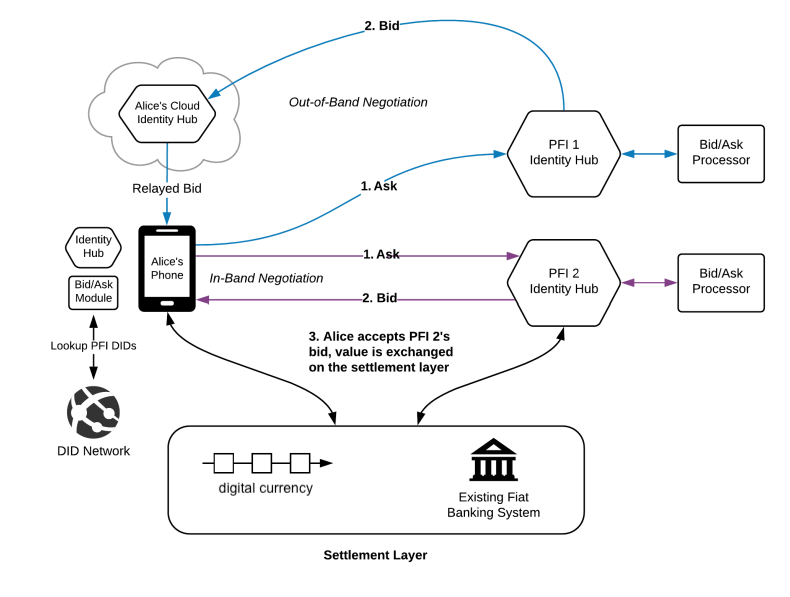
\includegraphics[width=15.61cm,height=11.83cm]{./diagrams/topology.png}{\small \textit{Topología y flujo de comunicación a nivel general}}
\end{center}


\vspace{1\baselineskip}
\subsection{Esquema de Mensajería Punto a Punto}

\vspace{1\baselineskip}
Los mensajes intercambiados entre los propietarios de billeteras y las PFIs que se transmiten entre los Nodos Web Descentralizados de los participantes contienen objetos definidos semánticamente adheridos a esquemas estándar. Estos objetos de mensaje definen todos los caminos del flujo ASK / BID / Liquidación y contienen los datos necesarios para que las contrapartes evalúen solicitudes, verifiquen credenciales y ejecuten intercambios de valor.

\vspace{1\baselineskip}
Los mensajes son objetos JSON, firmados por la parte que envía a la parte receptora para cada etapa de un intercambio, y pueden ser cifrados dependiendo del flujo o contenido que contienen. Existen ganchose que permiten a un servicio de manejo de mensajes recibir los mensajes a medida que llegan a un DWN y procesarlos de acuerdo con la semántica y el conjunto de reglas que el protocolo define para un tipo de mensaje dado.

\vspace{1\baselineskip}
\subsection{Descubrimiento de PFIs}

\vspace{1\baselineskip}
Para que las billeteras inicien y realicen intercambios de valor con PFIs, deben estar al tanto de los DIDs de las PFIs que desean incluir en su grupo de contrapartes potenciales. La conciencia de los DIDs de las PFIs permite a las billeteras resolver el conjunto de claves actual y los puntos finales de enrutamiento de DWN asociados con un DID dado. Prevemos varios medios para obtener conocimiento de los DID de las PFIs:

\vspace{1\baselineskip}
{\Large \textcolor[HTML]{434343}{Listas Curadas Individualmente}}

Los individuos pueden incluir cualquier entidad que deseen en sus listas de contrapartes deseadas. Las billeteras deben exponer funcionalidades e interfaces de usuario que faciliten este proceso de manera simple y comprensible para sus consumidores.

\paragraph{Listas Creadas por el Proveedor}

La forma más básica de inclusión de PFIs en el grupo de contrapartes potenciales de una billetera es la compilación de una lista de DIDs de PFIs por parte del proveedor de la billetera. Los proveedores de billeteras evaluarán los DIDs de las PFIs para su inclusión en sus listas basándose en sus propios criterios, que pueden incluir una combinación de procesos programáticos y humanos, como la inspección de VCs o procedimientos de verificación más tradicionales entre empresas.

\paragraph{Rastreo N-Grado de Listas de Proveedores}

Un participante en el ecosistema puede localizar una lista de DIDs confiable de otra entidad y elegir evaluar los DIDs incluidos de acuerdo con sus propios procesos de verificación. Una vez que se digiere un conjunto de DIDs, un participante puede optar por utilizar los DIDs de la lista para rastrear el siguiente nivel de listas que esos DIDs puedan ofrecer para su consideración.

\paragraph{Rastreo del Directorio DID}

Algunas implementaciones de DID proporcionan mecanismos para iterar el espacio del directorio DID dentro de ellas. Para implementaciones que ofrecen esta capacidad, los participantes pueden optar por rastrear el espacio más amplio del directorio DID y solicitar credenciales que establezcan confianza y/o listas de DIDs confiables desde los Nodos Web Descentralizados de las entidades que elijan responder.

\vspace{1\baselineskip}
En última instancia, corresponde a la billetera determinar qué lista de DID y qué PFIs confiar.

\vspace{1\baselineskip}
\subsection{Transacciones}

\subsubsection{Supuestos Técnicos}

Los siguientes son precondiciones necesarias para los flujos de protocolo descritos a continuación:

\begin{itemize}
	\item Los propietarios de billeteras y las PFIs poseen DIDs.

	\item Los propietarios de billeteras y las PFIs tienen Nodos Web Descentralizados vinculados a sus DIDs.

	\item Los propietarios de billeteras, a través de sus billeteras, pueden localizar PFIs mediante una conciencia curada de sus DIDs (listas generadas por la billetera) y/o rastreo y descubrimiento dinámico.

	\item Los propietarios de billeteras pueden encontrar y adquirir las VCs requeridas que las PFIs probablemente solicitarán.

\vspace{1\baselineskip}
\end{itemize}
A continuación se muestran ejemplos de escenarios de rampa de entrada (moneda fiduciario $\rightarrow$ moneda digital) y rampa de salida (moneda digital $\rightarrow$ moneda fiduciario), usando a Alice como un marcador de posición para representar a cualquier individuo que utilice el protocolo. Para el propósito de este ejemplo, utilizaremos USD, aunque el protocolo no se limita solo a USD.

\subsubsection{Ejemplo de Rampa de Entrada}

\begin{itemize}
	\item La billetera de Alice resuelve y almacena en caché el conjunto actual de claves y puntos de enlace DWN para los DIDs de las PFIs conocidas y descubiertas. Esta es una actividad periódica que la billetera repite según sea necesario.

	\item A través de la interfaz de usuario de la billetera, Alice inicia un flujo para solicitar moneda digital \textit{XYZ} a cambio de 100.00 USD.

	\item La billetera genera un mensaje semántico que refleja un \textit{ASK}, codificado con los parámetros de la solicitud de Alice.

	\item La billetera envía el mensaje \textit{ASK} a los Nodos Web Descentralizados de cada PFI que desea incluir como contraparte potencial de cumplimiento.

	\item Una PFI interesada responde al \textit{ASK} que recibe con una lista de \textit{BID}s.\textit{ Nota: La PFI tiene la libertad de elegir qué tipos de credenciales requiere para un BID dado, y es posible que la PFI ofrezca un BID sin requisitos de credenciales. Dado que cada VC adicional presumiblemente reduce el riesgo asumido por la PFI, es probable que las PFIs proporcionen mejores tasas o velocidades para BIDs con niveles más altos de requisitos de credenciales.}

	\item Alice elige uno de los BIDs respondiendo con el hash firmado original de ese \textit{BID}, junto con una presentación de las credenciales requeridas por ese \textit{BID}.

	\item El PFI verifica la presentación de Alice junto con las credenciales dentro de esa presentación y, si todo está en orden, envía un \textit{BID} final a Alice.

	\item Alice acepta el \textit{BID} firmándolo y enviándolo de vuelta a la PFI.

	\item El PFI publica un contrato inteligente en una blockchain y lo financia (para establecer prueba de capacidad de liquidación) con la cantidad acordada de moneda digital \textit{XYZ} y envía la dirección de la transacción a Alice.

	\item La billetera de Alice consulta el contrato para asegurar que la cantidad acordada esté presente. Luego, la billetera de Alice obtiene el medio de pago fiduciario aceptado desde el centro de la PFI. (El medio de pago fiduciario se expondrá como servicios individuales.) Alice selecciona su medio de pago preferido de los disponibles. La billetera de Alice facilita el pago a través del servicio asociado con el medio de pago seleccionado.

	\item Una vez que el PFI está satisfecha con el estado del pago fiduciario (esto puede ser cuando el pago se liquide, o puede ser antes si el PFI decide asumir más riesgo), ejecutan el contrato inteligente para liberar la moneda digital a la dirección de la billetera de Alice.

\vspace{1\baselineskip}
\end{itemize}
\begin{center}
\textit{Diagrama de rampa de entrada}
\end{center}



\vspace{1\baselineskip}
\begin{figure}[H]
\centering
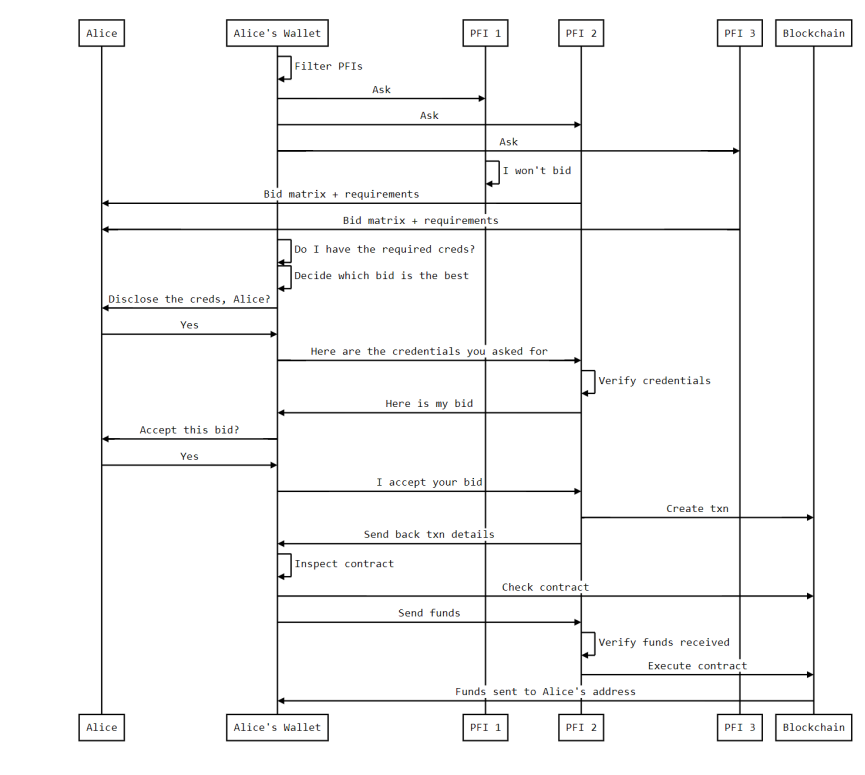
\includegraphics[width=16.4cm,height=15.3cm]{./diagrams/on-ramp.png}
\end{figure}

\subsubsection{Ejemplo de Rampa de Salida}

\begin{enumerate}
	\item La billetera de Alice resuelve y almacena en caché el conjunto actual de claves y puntos finales DWN para los DIDs de los PFIs conocidos y descubiertos. Esta es una actividad periódica que la billetera repite según sea necesario.

	\item A través de la interfaz de usuario de la billetera, Alice inicia un flujo para solicitar moneda fiduciario (en este caso USD) a cambio de 100 unidades de la moneda digital \textit{XYZ}.

	\item La billetera de Alice genera un mensaje semántico que refleja un \textit{ASK}, codificado con los parámetros de la solicitud de Alice.  

	\item La billetera de Alice envía el mensaje \textit{ASK} a los Nodos Web Descentralizados de cada PFI que desea incluir como contraparte potencial para el cumplimiento.

	\item Un PFI interesado responde al \textit{ASK} que recibe con una lista de \textit{BID}s. 

	\item Alice elige uno de los BIDs respondiendo con el hash firmado original de ese \textit{BID}, junto con una presentación de las credenciales requeridas por ese \textit{BID}. 

	\item El PFI verifica la presentación de Alice junto con las credenciales dentro de esa presentación y, si todo está en orden, envía un \textit{BID} final a Alice.

	\item Alice acepta el BID firmándolo y enviándolo de vuelta al PFI.

	\item La billetera crea un contrato inteligente y lo financia con 100 unidades de la moneda digital XYZ y envía la dirección del contrato al PFI.

	\item El PFI consulta el contrato inteligente para asegurar que la cantidad acordada de \textit{XYZ} esté presente y luego inicia una transacción para retirar los fondos a su billetera.

	\item El PFI envía la cantidad acordada de moneda fiduciario al destino proporcionado por Alice.

\vspace{1\baselineskip}
\end{enumerate}
Una de las motivaciones detrás de la introducción de un contrato inteligente es permitir que la moneda digital mantenida en el contrato inteligente se libere automáticamente de nuevo a Alice después de que haya transcurrido un cierto tiempo, en caso de que el PFI se desconecte y no cumpla con sus obligaciones.

\vspace{1\baselineskip}
El intercambio de valor real en los dos últimos pasos del ejemplo de salida pone más riesgo en Alice, ya que el PFI puede retirar la moneda digital de Alice antes de iniciar un envío de moneda fiduciario al destino proporcionado por Alice. \textcolor[HTML]{202124}{Idealmente, habría una forma de garantizar que el PFI enviará la moneda fiduciario antes de recibir la moneda digital.} En implementaciones futuras, los PFIs y las billeteras pueden confiar en servicios de monitoreo bancario y actuar como oráculos dentro del contrato inteligente para monitorear la cuenta bancaria del individuo y activar la liberación de fondos en moneda digital al PFI solo \textit{después} de que vean que se ha iniciado el envío de moneda fiduciario\textcolor[HTML]{3C4043}{.}

\vspace{9\baselineskip}
\begin{center}
\textit{\textcolor[HTML]{3C4043}{Diagrama de salida}}
\end{center}

\vspace{1\baselineskip}
\textcolor[HTML]{3C4043}{\begin{figure}[H]
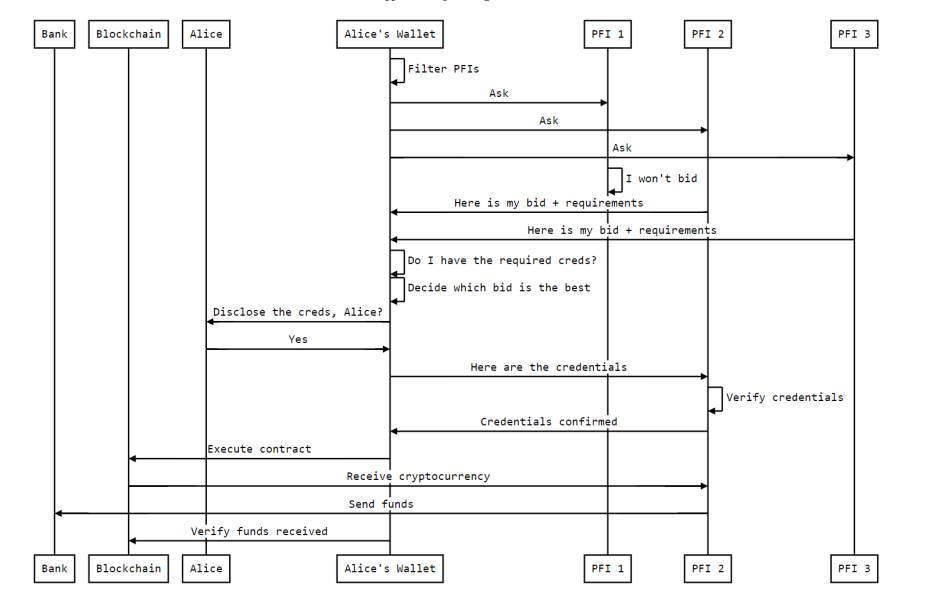
\includegraphics[width=15.48cm,height=10.29cm]{./diagrams/off-ramp.png}
\end{figure}
}

\vspace{1\baselineskip}
\subsubsection{Propiedades de un ASK}

En el ejemplo anterior, la billetera solicitante transmitirá un mensaje \textit{ASK} a los PFIs que contiene información clave requerida para evaluar la naturaleza del \textit{ASK}. Esto está destinado a ser a alto nivel para ayudar con la comprensión; la especificación final del protocolo puede diferir algo: \ \ 

\subparagraph{DID del Propietario de la Billetera}

El DID asociado con el propietario de la billetera (ya sea un individuo o una institución).

\subparagraph{Tipo de Activo Deseado}

El tipo de activo solicitado (por ejemplo, TOKEN-USDC, TOKEN-BTC, TOKEN-MXN, FIAT-USD, FIAT-EUR, etc.), donde los activos precedidos por TOKEN son activos de moneda digital, y los activos precedidos por FIAT son monedas fiduciarios.\textit{ }

\subparagraph{Cantidad de Activo Deseada}

La cantidad de activos deseados solicitados. Esto puede estar vacío si se desea una cotización para una cantidad ofrecida. 

\subparagraph{Esquema de Liquidación Deseado}

El mecanismo mediante el cual se solicita la liquidación. Esto permitirá a una billetera especificar qué cadena de bloques o protocolo utilizar para efectuar la liquidación. Por ejemplo, muchos stablecoins existen en múltiples cadena de bloques, y bitcoin se puede liquidar en soluciones de capa dos como Lightning. Para las monedas fiduciarios, los protocolos de liquidación podrían incluir mecanismos como SEPA, ACH, Tarjetas de Pago, SWIFT, entre otros.

\subparagraph{Tipo de Activo Ofrecido}

El tipo de activo propuesto para el pago. Los mismos valores de campo que 'Tipo de Activo Deseado'.

\subparagraph{Esquema de Liquidación Ofrecido}

El esquema de liquidación para el tipo de activo ofrecido. Los mismos valores de campo que ‘Esquema de Liquidación Deseado’.

\subparagraph{Cantidad de Activo Ofrecido}

La cantidad de activos deseados ofrecidos. Vacío si se desea una cotización por la cantidad propuesta por el PFI. 

\vspace{1\baselineskip}
\subsubsection{Propiedades de un BID}

Una oferta de un PFI a la billetera contendrá elementos que describen la propuesta para una transacción de intercambio, que incluye ofertas sobre el precio, credenciales requeridas y parámetros de liquidación. 

\subparagraph{PFI DID}

El DID asociado con el PFI. 

\subparagraph{Costo Propuesto (en Tipo de Activo Ofrecido del ASK)}

El costo propuesto para la transacción denominado en el \textit{Tipo de Activo Ofrecido} del mensaje ASK. No se devuelve si se especificó la \textit{Cantidad de Activo Ofrecido}. 

\subparagraph{Cantidad Propuesta para Liquidación (en Tipo de Activo Deseado del ASK)}

La cantidad propuesta para liquidar la transacción denominada en el \textit{Tipo de Activo Deseado} del mensaje ASK. No se devuelve si se especificó la \textit{Cantidad de Activo Deseado}. 

\subparagraph{Tiempo de Liquidación}

El tiempo máximo (a partir del momento en que se acepta la oferta) en el que se efectuará la liquidación. Después de este tiempo, se presupondrá que ha ocurrido un incumplimiento de la liquidación. 

\subparagraph{Expiración de la Oferta}

El tiempo después del cual la oferta se considerará obsoleta y ya no será válida por el PFI. 

\subparagraph{Firma}

Una firma sobre los parámetros del BID generada por la clave privada del PFI, para protección de la integridad. 

\vspace{2\baselineskip}
\section{Confianza en la Reputación}


\vspace{1\baselineskip}
Las billeteras y los PFIs negocian la confianza directamente entre sí, y pueden depender de terceros mutuamente confiables para avalar a las contrapartes. El protocolo y la red en sí no proporcionan ninguna consideración especial a los terceros confiables; estas relaciones deben establecerse a través de procesos programáticos y humanos ortogonales.

\vspace{1\baselineskip}
Por ejemplo, el implementador de una billetera puede optar por ensamblar y publicar \textit{listas que expresan sentimientos positivos o negativos} sobre los DIDs de los PFI\textit{s} que están incluyendo o excluyendo de sus ofertas. Esto es similar a cómo los proveedores de navegadores web incluyen listas de Autoridades Certificadoras (CAs) pre-cargadas para establecer una base de confianza para la Seguridad de la Capa de Transporte (TLS), que se utiliza para asegurar las transferencias de datos en la web.

\\ La capacidad de revocar o modificar el estatus de un DID en una \textit{lista de sentimientos} es un elemento recomendable para cualquier esquema de este tipo, similar a la revocación de certificados con CAs. Esto podría implementarse de manera robusta utilizando VCs y mecanismos de publicación DWN. El diseño exacto de dicho esquema está más allá del alcance de este documento, pero es un componente importante que buscamos resolver a medida que operacionalizamos este protocolo.

\vspace{1\baselineskip}
\section{Riesgos y Consideraciones Adicionales}

\vspace{1\baselineskip}
{\LARGE Riesgos $\&$ Consideraciones para PFIs}

\vspace{1\baselineskip}
Los PFIs regulados están sujetos a requisitos y obligaciones impuestos por ley, como la supervisión y prevención de actividades de lavado de dinero en sus plataformas y garantizar que no estén involucrados con terroristas o individuos sancionados. Más allá de las obligaciones y riesgos regulatorios, los PFIs también deben gestionar riesgos financieros, incluidos los relacionados con contracargos, fraudes e incumplimientos. Los riesgos para los PFIs se dividen en tres categorías amplias: delitos financieros; contracargos / fraudes; y suscripción / incumplimientos.

\subsubsection{Delitos Financieros}

Las instituciones financieras gestionan estos riesgos desarrollando programas robustos de cumplimiento AML y antiterrorista para monitorear actividades ilícitas. En el ámbito de las monedas digitales, muchos PFIs han tomado el paso adicional de aprovechar soluciones de análisis de cadenas de bloques y análisis cruzado de cadenas para decidir con qué individuos o billeteras interactuar y qué transacciones facilitar.

\vspace{1\baselineskip}
De acuerdo con la implementación del protocolo tbDEX, el uso de soluciones de análisis blockchain e inteligencia puede ayudar a los PFIs a filtrar, puntuar y monitorear billeteras individuales y transacciones para evaluar transacciones basadas en el criterio de riesgo del PFI y las obligaciones regulatorias. Más allá de detectar y evaluar el riesgo de delitos financieros, las soluciones de análisis blockchain también pueden emplearse para proporcionar puntuaciones de riesgo basadas en transacciones anteriores como parte de un esquema de vigilancia post-transacción para detectar riesgos con entidades previamente encontradas.

\subsubsection{Contracargos / Fraude}

Un contracargo es un pago con tarjeta de crédito o débito que es revertido por un banco en favor del titular de la tarjeta después de que el pago ha sido procesado y liquidado. Los contracargos ocurren cuando un cliente solicita a los bancos que devuelvan sus fondos por una variedad de razones, siendo la más común la no entrega de bienes o servicios, o el uso no autorizado de tarjetas de pago. En el contexto del protocolo tbDEX, los contracargos presentan un desafío adicional porque la tarjeta de crédito o débito se usa para comprar moneda digital que luego puede ser depositada en una billetera de autocustodia, donde los activos no pueden ser recuperados por los PFIs. En este ejemplo, hay una asimetría entre un instrumento de pago reversible en el mundo fiduciario frente una transacción no reversible o recuperable en el mundo de las monedas digitales. Encontrar cómo gestionar eficazmente los riesgos de fraude y contracargos es un área significativa para el desarrollo futuro que buscaremos abordar en versiones futuras del documento.

\subsubsection{Suscripción / Incumplimientos}

Otra consideración para los PFIs es si el propietario de la billetera es ``bueno" para los fondos prometidos en la transacción. Este es un problema particularmente agudo para los sistemas bancarios en todo el mundo que se basan en sistemas de pagos de capa base heredados que impiden a los bancos operar cuentas en un modelo de ``fondos buenos" que asegura que los saldos no puedan ser negativos. Como ejemplo, el sistema de cámara de compensación automatizada (ACH) utilizado para el procesamiento de cheques en los Estados Unidos es un sistema de procesamiento por lotes de ``dispara y olvida" a través del cual las transacciones regularmente tardan varios días hábiles en liquidarse. En el interín de tres a cinco días hábiles, las transacciones ACH pueden ser rechazadas por una serie de razones, incluidos fondos insuficientes, cheques devueltos y cuentas cerradas. En todos estos ejemplos, los fondos nunca serán recibidos por el destinatario previsto de la transacción ACH.

\vspace{1\baselineskip}
En el contexto de los intercambios que ocurren a través del protocolo \textit{tbDEX}, los PFIs están sujetos a riesgo de crédito mientras sea posible que los saldos se vuelvan negativos porque los fondos subyacentes que se prometieron salen de la cuenta designada antes de que la transacción se liquide. Esto es especialmente cierto para los PFIs que buscan ofrecer transacciones aceleradas para apoyar una experiencia de usuario casi en tiempo real al enviar monedas estables a las billeteras después de que se inicie la transacción ACH, pero antes de que se liquide.

\vspace{1\baselineskip}
Mientras que esta es la razón por la cual los bancos y otras instituciones financieras suscriben clientes potenciales en el mundo financiero tradicional (y se niegan a bancar clientes que consideran un riesgo crediticio), hay otras razones por las cuales pueden ocurrir incumplimientos, incluida la falla de la transacción misma después de que la moneda digital haya sido enviada a una billetera de autocustodia. Aunque es posible que los PFIs ajusten el precio de sus ofertas en función de su percepción del riesgo de incumplimientos o contracargos, estos escenarios son temas que deben abordarse con mayor detalle en versiones futuras del documento.

\vspace{1\baselineskip}
\subsection{Riesgos y Consideraciones para Billeteras}

\subsubsection{Suplantación de identidad}

Un ataque potencial grave que podría organizarse contra las billeteras sería un nodo PFI que se haga pasar por un nodo legítimo de entrada y salida fiduciario, con la intención de capturar información personal identificable (PII) o credenciales financieras con el propósito de obtener información de manera ilegítima para el robo de identidad o financiero. La primera línea de defensa contra estos tipos de ataques depende en gran medida de la verificación de confianza a través de VCs compartidos mutuamente. Por lo tanto, las implementaciones de billeteras y los operadores de billeteras serían altamente recomendados a emplear listas de nodos PFI confiables que puedan ser verificadas de manera independiente. En ausencia de esto, se alentaría al operador de la billetera a realizar una investigación y verificación independiente de la confiabilidad de la contraparte antes de comprometerse a transmitir información sensible.

\subsubsection{Incumplimiento de Liquidación / No Entrega de Fondos}

Después de entrar en un contrato, también es posible que un PFI pueda fallar en la entrega de fondos por razones no relacionadas con fraude o mala conducta. Esta es un área que se abordará en futuras revisiones del documento. Direccionalmente, el uso de identidades verificadas para PFIs crea la oportunidad para procesos de disputa fuera de banda utilizando medios legales u otros. Este escenario también puede abordarse a través de información públicamente referenciable sobre incumplimientos utilizando liquidación en depósito basada en contratos inteligentes, o un protocolo de torre de vigilancia separado. \ \ \ \ \ \ \ \ \ \ \ \ \ \ \ \ \ \ \ \ \ \ \ \ \ \ \ \ \ \ \ \ \ \ \ \ \ \ \ \ \ \ \ \ \ \ \ \ \ \ 

\vspace{1\baselineskip}
\section{Nota sobre Anonimato y Resistencia a la Censura}

\vspace{1\baselineskip}
El documento de Bitcoin [5] delineó una visión para una moneda digital nativa y un sistema de pagos sin necesidad de confiar en terceros. Este es un atributo fundamental que proporciona las propiedades de resistencia a la censura, acceso universal y seguridad.

\vspace{1\baselineskip}
Cuando el mundo digital interactúa con el mundo físico, las garantías sin confianza no cruzan la división. Aunque es cierto que, por ejemplo, una transacción de bitcoin entre billeteras no requiere un tercero confiable o intermediario, también es cierto que en los pagos por bienes y servicios, el riesgo de contraparte sigue existiendo. Con bitcoin, el beneficiario puede recibir fondos sin la posibilidad de que el pagador incumpla su obligación financiera, pero el beneficiario aún puede incumplir la transacción por no entregar los de bienes o servicios. Un par físico de calcetines no puede intercambiarse atómicamente con bitcoin en un DEX. De hecho, es imposible e irrazonable esperar que tal transacción pueda llevarse a cabo puramente de forma anónima, sin que las contrapartes tengan alguna relación de confianza externa. En el caso promedio, el beneficiario necesita una dirección de envío física, mientras que el pagador buscaría alguna señal para confiar en que el beneficiario es un negocio legítimo.

\vspace{1\baselineskip}
El intercambio de moneda fiduciario y digital sufre del mismo problema. ¿Se puede confiar en la contraparte para entregar moneda fiduciario a cambio de moneda digital? ¿Cuáles son las consecuencias si no lo hacen?

\vspace{1\baselineskip}
El protocolo \textit{tbDEX} busca utilizar sistemas de identidad descentralizada con VCs para crear mercados de confianza, a través de terceros mutuamente elegidos. Esto puede percibirse como un intento de socavar el anonimato o ``desanonimizar" las transacciones. Pero también debemos reconocer que, por las razones mencionadas anteriormente, el anonimato para transacciones de bienes y servicios tiene un costo: riesgo de contraparte sin límites.

\vspace{1\baselineskip}
Así, nuestro objetivo es la resistencia a la censura, el acceso sin permisos y la maximización de la competencia por la liquidez \textcolor[HTML]{202124}{— }con el objetivo final de commoditizarla alrededor del mundo. Nuestro objetivo no es mantener el anonimato de las transacciones a toda costa. Tampoco es socavar la capacidad de un individuo para optimizar el anonimato. Nada en principio impide las transacciones anónimas para la privacidad financiera en la red \textit{tbDEX}. Un PFI podría, en principio, no requerir VCs, pero tales transacciones representarían un alto grado de riesgo para las contrapartes.

\vspace{1\baselineskip}
\section{Tareas Pendientes}

\vspace{1\baselineskip}
Este borrador inicial del documento tiene como objetivo establecer una comprensión conceptual del diseño de alto nivel del protocolo \textit{tbDEX} propuesto. No debe \textit{considerarse} completo o final. Representa un diseño propuesto para comentario público.

\vspace{1\baselineskip}
Las revisiones futuras del documento abordarán elementos incompletos y problemas o desafíos actualmente no previstos.

\vspace{1\baselineskip}
Después de la aceptación del diseño final del protocolo, se desarrollará y publicará una \textit{Especificación del Protocolo tbDEX}. A continuación, se desarrollará una implementación de referencia de código abierto conforme a los estándares y SDK para billeteras, así como una implementación de referencia del software del Nodo PFI.

\vspace{1\baselineskip}
\section{Comentarios}

\vspace{1\baselineskip}
Nuestro objetivo es desarrollar esto como un proyecto de código abierto para el bien público. ¡Tenemos mucho trabajo por hacer! Existen numerosos desafíos asociados con la realización de \textit{tbDEX}, y hay muchas cosas que sabemos que aún tenemos que considerar. Agradecemos su aporte sobre cómo mejorar este documento.

\vspace{1\baselineskip}
Para enviarnos comentarios o ideas, por favor, tuitee a @TBD54566975 en \url{https://twitter.com/TBD54566975} o envíenos una solicitud de extracción en \url{https://github.com/TBDev-54566975/white-paper}{\Large .}

\vspace{1\baselineskip}
\section{Referencias}

[1] \textit{The Global Findex Database (2017)}, ``La Inclusión Financiera en Aumento, Pero Aún Existen Brechas, Muestra la Base de Datos Global Findex"; 19 de abril de 2018 del Grupo del Banco Mundial: \url{https://www.worldbank.org/en/news/press-release/2018/04/19/financial-inclusion-on-the-rise-but-gaps-remain-global-findex-database-shows} y \url{https://globalfindex.worldbank.org}.

\vspace{1\baselineskip}
[2] \textit{Identificadores Descentralizados (v1.0)}. Sporny, Longley, Sabadello, Reed, Steele, Allen; 3 de agosto de 2021 del World Wide Web Consortium (W3C): \url{https://www.w3.org/TR/did-core/}.

\vspace{1\baselineskip}
[3] \textit{Modelo de Datos de Credenciales Verificables (v1.1)}, ``Expresando Información Verificable en la Web", Sección 5.8 sobre Pruebas de Conocimiento Cero. Sporny, Noble, Longley, Burnett, Zundel; 9 de noviembre de 2021 del World Wide Web Consortium (W3C): \url{https://www.w3.org/TR/vc-data-model/#zero-knowledge-proofs}. \ \ 

\vspace{1\baselineskip}
[4] \textit{Credenciales de Conocimiento Cero con Comprobaciones de Revocación Diferidas}. Chase, Ghosh, Setty, Buchner; 13 de julio de 2020 de la Fundación de Identidad Descentralizada (DIF): \url{https://github.com/decentralized-identity/snark-credentials/blob/master/whitepaper.pdf}

\vspace{1\baselineskip}
[5] \textit{Bitcoin: Un Sistema de Dinero Electrónico Peer-to-Peer}. Satoshi Nakamoto; (s.f.) de Bitcoin.org: \url{https://bitcoin.org/bitcoin.pdf}.
\end{document}
